% Start - Hardware/Control Unit/Oscillator Circuit
%write Between the comments


\subsubsection{Oscillator Circuit}
%first create all the reference in bibfile.

	\paragraph{The} oscillator circuit is required for generating clock for \gls{mcu}.Accuracy of timing application is dependent on the accuracy of the oscillator provided in the \gls{mcu}. The oscillators supported by ATmega328P are listed below \cite{AtMega328P}.
		\begin{itemize}
			\item Low power crystal oscillator
			\item \textbf{Full swing crystal oscillator}
			\item Low frequency crystal oscillator
			\item Internal 128 \gls{khz} RC oscillator
			\item Calibrated internal RC oscillator
			\item External clock
		\end{itemize}		
		
	\subparagraph{For }
	this application the \gls{mcu} will be in Full swing crystal oscillator mode.
	
	\subparagraph{\textbf{Advantages:}}
		
		\begin{itemize}
			\item 16 \gls{mhz}.
			\item rail to rail swing.
			\item Drive other clock sources
			\item Less effect of noisy environment 
		\end{itemize}		
	 
	 \subparagraph{Disadvantages:}
	 
	 	\begin{itemize}
	 		\item Higher current consumption than Low power crystal oscillator.(Power consumed by a crystal is not very significant, since using a 230 V AC source.)
	 		\item Operating Voltage of \gls{mcu} becomes 2.7 V to 5.00 V.(\gls{mcu} will be working on 5 V DC which is within the operating voltage defined.) 
		\end{itemize}	  	  
		
	\textbf{Selecting Crystal}
	
	\paragraph{Crystal Requirement}
	
		\begin{itemize}
			\item Frequency: 16 \gls{mhz}
			\item $C_{L}$: 6 - 11 pF \cite{AtMega328P}
			\item Mode of operation : Fundamental 
			\item Resonant: Parallel
			\item Tolerance: 0 - 50 \acrshort{ppm}
			\item Temperature Stability: 0 - 50 \acrshort{ppm}
			\item \gls{esr}: 60 to 100 $\Omega$
			\item Package type : \gls{smt} , since such crystals provide with less stray capacitance.
		\end{itemize}
	
	\paragraph{Selected Crystal} 
	is TSX-3225 16.0000MF09Z-AC0 a \gls{smt} 4 pin device package. Refer \ref{tab:selected_crystal} for details. 

	\subparagraph*{Oscillator Circuit Design}
	
		\begin{enumerate}
			\item \textbf{Load Cpacitors}:
			
				\begin{itemize}
					\item $C_{1}$ and $C_{2}$ together act as load capacitance.			
	
	\begin{figure}[H]
		\caption{Oscillator Circuit}
		\label{fig:crystal_circuit}
		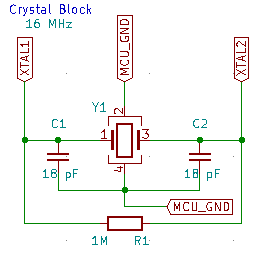
\includegraphics[scale=1]{crystal_ckt.png}
	\end{figure}

	\begin{table}[H]
		\caption{Crystal Properties(cite datasheet)}
		\label{tab:selected_crystal}
		\begin{tabular}{|r|c|}
				\hline
				\textbf{Device Manufacturer}                                                                            & \textbf{EPSON}                                                                            \\ \hline
				\textbf{Part No.}                                                                                       & \multicolumn{1}{l|}{\begin{tabular}[c]{@{}l@{}}TSX-3225 16.0000\\ MF09Z-AC0\end{tabular}} \\ \hline
				\textbf{Case (mm X mm)}                                                                                 & 3.2 x 2.5                                                                                 \\ \hline
				\textbf{\acrshort{tht} / \gls{smt}}                                        & SMD                                                                                       \\ \hline
				\textbf{\begin{tabular}[c]{@{}r@{}}Fundamental \\ Frequency ( \gls{mhz})\end{tabular}} & 16                                                                                        \\ \hline
				\textbf{\begin{tabular}[c]{@{}r@{}}Frequency \\ Stability (\acrshort{ppm})\end{tabular}}    & 9                                                                                         \\ \hline
				\textbf{\begin{tabular}[c]{@{}r@{}}Frequency \\ Tolerance(\acrshort{ppm})\end{tabular}}     & 10                                                                                        \\ \hline
				\textbf{$C_{L}$ pF}                                                                                     & 9                                                                                         \\ \hline
				\textbf{\begin{tabular}[c]{@{}r@{}}Operating\\ Temp max(\textdegree C )\end{tabular}}        & 75                                                                                        \\ \hline
				\textbf{\begin{tabular}[c]{@{}r@{}}Operating \\ Temp min(\textdegree C)\end{tabular}}        & -20                                                                                       \\ \hline
				\textbf{Aging (\acrshort{ppm})}                                                             & 1                                                                                         \\ \hline
				\textbf{ESR ($\Omega$)}                                                                                 & 60                                                                                        \\ \hline
		\end{tabular}
	\end{table}
	
	\item To have total 180\textdegree 	 shift due to active components (i.e capacitors), each capacitor provides with 90\textdegree  shift in phase. The value of the load capacitor is provided (cite datatsheet). 
	\item $C_{L}$ (Total Load capacitance) = 9 pF (cite DS)
	\item $C_{s}$ : Stray capacitance.
	\item $C_{1}$, $C_{2}$ are load capacitors
	\item Considering $C_{1} = C_{2}$. 
	\item value of $C_{1}$ and $C_{2}$ can be calculated using the following equation.
					\begin{align}				
						C_{L} &= {\frac{C_{1}C_{2} }{C_{1} + C_{2}}} + C_{s}\\
						C_{1} &= 2(C_{L} - C_{s})			
					\end{align}
	\item Considering $C_{s}$ = 0 pF.
					\begin{align}
						C_{1} &= 2(9 - 0)\\
						C_{1} &= 18 pF
					\end{align}
	\item Since crystal has drive level in range of 200 $\mu$ W, 0603 package ,i.e 0.1 W, is selected with value of 18 pF, 0603.
	\item The resistor $R_{1}$ is used to make the behaviour linear, this enhances the output of the crystal circuit. $R_{1}$ = 1 M $\Omega$, 0603.
				\end{itemize}
		
		\end{enumerate}		
	\paragraph{\gls{pcb} } design.
	

\cite{AVR042}

% End - Hardware/Control Unit/Oscillator Circuit